\chapter{Institutions as Story Worlds}
\label{cha:institutions}

% Intro about justification/inspiration for using institutions for stories

\section{Describing Stories With Logic}
Section~\ref{sec:model-logic} describes approaches that use formal logic to model interactive, non-linear narratives. Building on the work described in that section, we explore other possible ways with which to construct these kinds of stories.

% Describe why we will build stories with Propp and tropes (as a method of comparison)

\subsection{Modal Logic and Kripke Structures}

\subsubsection{Propp Example: Sausages and Crocodile Scene}\label{sec:pjexample}
The common elements of Punch and Judy are easily described in terms of Propp's story functions. Here we pick one scene to use as an example: the scene where Punch battles a Crocodile in order to safeguard some sausages.  In this scene, Joey the clown (our narrator) asks Punch to guard the sausages. Once Joey has left the stage, a Crocodile appears and eats the sausages. Punch fights with the Crocodile, but it escapes. Joey then returns to find that his sausages are gone.
The corresponding story functions are:
\begin{compactenum}
  \item Joey tells Punch to look after the sausages (\emph{interdiction}).
  \item Joey has some reservations, but decides to trust Punch (\emph{complicity}).
  \item Joey gives the sausages to Punch (\emph{provision or receipt of a magical agent}).
  \item Joey leaves the stage (\emph{absentation}).
  \item A Crocodile enters the stage and eats the sausages (\emph{violation}).
  \item Punch fights with the Crocodile (\emph{struggle}).
  \item Joey returns to find that the sausages are gone (\emph{return}).
\end{compactenum}

Some story functions map to Punch and Judy better than others (for example, it is debatable as to whether or not the sausages can be considered a ``magical agent''), but Propp's formalism seems well suited to Punch and Judy for the most part. The advantage of using Propp for the Punch and Judy story domain is that the story function concept maps well to the idea of internal events in institutional models.

\subsubsection{Combining Interval Temporal Logic and Modal Logic for Propp}\label{sec:propplogic}
\mnote{Put in definitions as a footnote, Cyrillic if you want}
Narrative construction can be described using two terms: \emph{fabula} and \emph{syuzhet}. Fabula is the events of the story as they occur in chronological order, but syuzhet refers to those events as they are ordered in the story's telling. Fabula describes one event following another, but syuzhet could describe events occuring out of order, branching sequences and events that occur at the same time.

The challenge faced here is how to find a way of not only describing the syuzhet of one story, but of all possible stories and paths through a story in a narrative world.

\paragraph{Modal Logic}
Modal logic extends classical propositional and predicate logic with modalities, which are operators that qualify a statement. For example, rather than simply stating `The Crocodile eats the sausages', we could instead say ``the Crocodile sometimes eats the sausages'', or ``it's possible that the Crocodile eats the sausages''.
Classic modal logic deals with \emph{alethic modality}, which describes whether a statement is \emph{possible} or \emph{necessary}. This is implemented using unary operators to qualify statements. For example, $\Diamond P$ states that $P$ is possible and $\Box P$ states that $P$ is necessary.
Naturally, we can use modalities beyond just possibility and necessity. In order to describe the syuzhet of a story, we need to be able to make statements such as ``The Crocodile eats the sausages at the beginning of the scene'', and ``Punch kills the baby while before his wife returns''. For this, we turn to \emph{temporal logic}.

\mnote{Why use modal logic for possible worlds?}

\paragraph{Temporal Logics}
Arthur Prior is the first to employ modal logic as a way of describing sequences of time in his 1957 work \emph{Time and Modality} \cite{prior2003time}. Here he uses just two modal operators, $P$ and $F$, representing \emph{some time in the past} and \emph{some time in the future} respectively.
Hans Kamp adds two extra operators to Prior's logic, \emph{Since} and \emph{Until}, in his 1968 thesis \cite{kamp1968tense}, enabling it to describe spans of time in addition to the ordering of temporal events.
As Kripke later points out to Prior, this model lacks the expressiveness needed to describe all possible sequences of events. One major shortcoming is its restriction to describing only \emph{linear} events. 

Linear Temporal Logic (LTL), though still limited to the description of linear sequences of events, is an evolution of the work done by Prior and Kamp. Proposed by Amir Pnueli in 1977 \cite{pnueli1977temporal}, its original use is for the formal verification of computer programs.
Computational Tree Logic (CTL) \cite{ben1983temporal} is similar to LTL, but allows for the representation of non-linear time through the allowance of branches. Through CTL it is possible to describe several alternative pathways through time, though only one may ever be actualised. Like LTL, its original purpose is for formal verification of software, and in model checkers.
Both CTL and LTL are subsets of CTL* (Computational Tree Logic) \cite{emerson1986sometimes}, which can both describe both multiple branches of temporal paths and their durations. CTL* formulae must refer to a specific Kripke structure, however (a description of Kripke structures appears in section \ref{sec:kripke}).

\paragraph{Interval Temporal Logic}
In order to model fabula with modal logic, we employ Interval Temporal Logic (ITL), composed of the temporal intervals defined by Allen \cite{allen1983maintaining} and developed into modal operators by Halpern and Shoham \cite{halpern1991propositional}. This allows the expressiveness necessary to describe branching, parallel and nested paths through stories.

In most temporal logics (such as CTL* and its subsets), fixed \emph{time points} without duration are the basic unit of time. However, this can make it difficult to reason about the \emph{duration} of events that occur over a period of time. Temporal Interval Logic tackles this problem through the use of \emph{time intervals} or \emph{periods} as the basic temporal unit.

The version of ITL used here is that described by Della Monica et al. in their overview paper \cite{della2013interval}. Table \ref{tab:itl} lists the temporal intervals described by Allen, along with their modal operator equivalents in \emph{Halpern-Shoham logic}.

The operators defined by Halpern and Shoham are (a bar over an operator denotes its inverse):

\begin{compactitem}
\item $\langle L \rangle / \langle \overline{L} \rangle$ (Later): The interval occurs at some point after another interval.
\item $\langle A \rangle / \langle \overline{A} \rangle$ (After): The interval occurs immediately after another interval.
\item $\langle O \rangle / \langle \overline{O} \rangle$ (Overlaps): The interval occurs both during and before or after another interval.
\item $\langle E \rangle / \langle \overline{E} \rangle$ (Ends): The interval ends at exactly the same time as another interval.
\item $\langle D \rangle / \langle \overline{D} \rangle$ (During): The interval both starts and ends inside the duration of another interval.
\item $\langle B \rangle / \langle \overline{B} \rangle$ (Begins): The interval begins at exactly the same time as another interval.
\end{compactitem}
\begin{table}[!t]
  \centering
  \caption{Operators in the Interval Temporal Logic (adapted from \cite{della2013interval})}
  \label{tab:itl}
  \begin{tabular}{l|l|l}
    {\bf Interval} & {\bf Allen notation} & {\bf HS notation} \\
    \hline& &\\
    \multirow{7}{*}{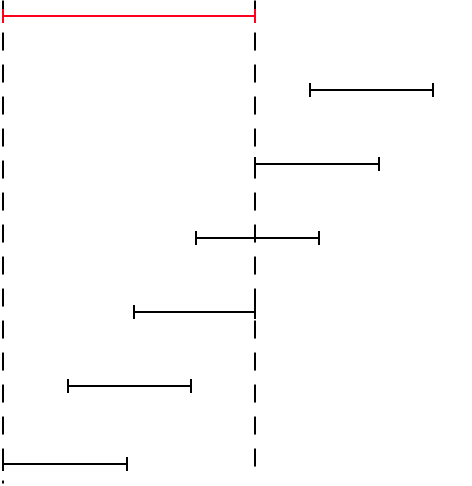
\includegraphics[height=2.02in]{intervals.png}}&\emph{equals} \{=\} &\\
    & &\\
                   &\emph{before} \{\textless\} / \emph{after} \{\textgreater\} & $\langle L \rangle$ / $\langle \overline{L} \rangle$ \emph{(Later)}\\
    & &\\
                   &\emph{meets} \{\emph{m}\} / \emph{met-by} \{\emph{mi}\} &$\langle A \rangle$ / $\langle \overline{A} \rangle$ \emph{(After)}\\
    & &\\
    &\emph{overlaps} \{\emph{o}\} / \emph{overlapped-by} \{\emph{oi}\} &$\langle O \rangle$ / $\langle \overline{O} \rangle$ \emph{(Overlaps)}\\
    & &\\
    &\emph{finished-by} \{\emph{fi}\} / \emph{finishes} \{\emph{f}\} &$\langle E \rangle$ / $\langle \overline{E} \rangle$ \emph{(Ends)}\\
    & &\\
    &\emph{contains} \{\emph{di}\} / \emph{during} \{\emph{d}\} &$\langle D \rangle$ / $\langle \overline{D} \rangle$ \emph{(During)}\\
    & &\\
    &\emph{started-by} \{\emph{si}\} / \emph{starts} \{\emph{s}\} &$\langle B \rangle$ / $\langle \overline{B} \rangle$ \emph{(Begins)}
  \end{tabular}
\end{table}
\subsubsection{Propp Example with Punch and Judy}
In this example, we combine Halpern and Shoham's temporal operators with the possibility ($\Diamond$) and necessity ($\Box$) operators of modal logic. We follow the convention of writing possibility operators inside angle brackets: $\langle \, \rangle$ and necessity operators within square brackets: $[ \, ]$.

This example shows the ``sausages'' scene described in section \ref{sec:pjexample}, consisting of a set of situations $S$, containing Propp story functions $P$. The interval temporal logic operators used in this example are the set $T$. Figure \ref{fig:operators} shows the modal operators we use. $A, B$ and $C$ in formula \ref{eq:story} are variables that represent the characters and objects that appear in the story.
\begin{figure}[!t]
\begin{align}
    S &= \{S_0, S_1, S_2, S_{3a}, S_{3a_1}, S_4, S_{3b}, S_{3b_1}, S_4, S_5\}\\
    P &= \{\mathtt{interdiction(A, B, C), absentation(A), struggle(A, B),}\nonumber\\
  &\qquad\qquad\mathtt{victory(A), villainy(A, B), violation(A, B), return(A)}\}\label{eq:story}\\
  T &= \{D, \overline{D}, O, \overline{O}, A, \overline{A}, B, \overline{B}, L, \overline{L}, E, \overline{E}\}
\end{align}
\caption{Modal operators}\label{fig:operators}
\end{figure}
Hybrid logics allow worlds, time intervals, to be named. The hybrid logic nominal operator allows specific times to be uniquely referenced, allowing a logic to talk about specific states such as $S_0..S_5$. The nominal proposition is true of one specific time interval such that any two worlds with the same name represent co-extensive intervals of time. Anything true of one is true of the other.
We also make use of a nominal modal operator so that it is possible to make assertions about these named worlds, ``It is necessary that in state $S_1$ Joey absents himself.'' This technique enables us to associate story functions with specific, named intervals.
We use hybrid logic to identify nodes using the \emph{nominal} operator, shown as $@$. The nominal operator adds the capability of referring to possible worlds in formulas. In this way, each possible state of a system can be labelled and referenced from other states. As seen in figure \ref{fig:lotrec}, each nominal node must have its own name as a relation leading back to the root node, in order to be linked to and referred from the other nodes.
We can combine this with the Interval Temporal Logic to make statements such as ``An absentation starts with state $@S_1$ and ends with state $@S_5$.'' (formula \ref{eq:absentation}).
Figure \ref{fig:situations} describes the full sausages scene from Punch and Judy using the time intervals shown in figure \ref{fig:durations}.
\begin{figure}[!t]
  \centering
    \centerline{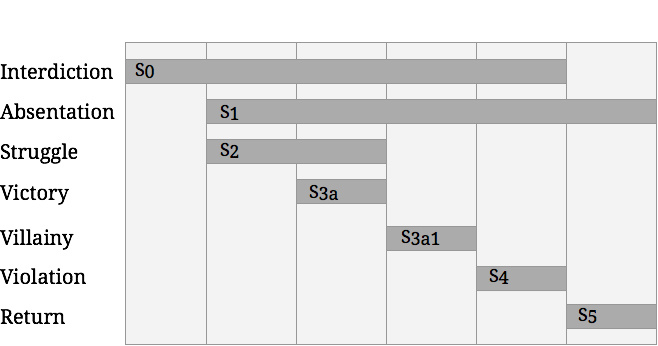
\includegraphics[width=0.9\textwidth]{durations.png}}
  \caption{Timings of the story functions in the sausages scene}\label{fig:durations}
\begin{align}
  &S_{0} \land \mathit{interdiction(Joey, Punch, Sausages)} \land\nonumber\\
  &\qquad\qquad\qquad\qquad\qquad\langle B \rangle @S_{1} \land \langle E \rangle @S_{4} \land \langle A \rangle @S_{5}\label{eq:interdiction}\\
  &[@S_{1}] \mathit{absentation(Joey)} \land \langle A \rangle @S_{2}\label{eq:absentation}\\
  &[@S_{2}] \mathit{struggle(Punch, Crocodile)} \land \langle E \rangle (@S_{3a} \lor @S_{3b})\label{eq:struggle}\\
  &[@S_{3a}] \mathit{victory(Crocodile)} \land \langle A \rangle @S_{3a_1}\\
  &[@S_{3a_1}] \mathit{villainy(Crocodile, Sausages)} \land \langle E \rangle @S_{4}\\
  &[@S_{3b}] \mathit{victory(Punch)} \land \langle A \rangle @S_{3b_1}\\
  &[@S_{3b_1}] \mathit{villainy(Punch, Sausages)} \land \langle E \rangle @S_{4}\\
  &[@S_{4}] \mathit{violation(Punch, Sausages)}\\
  &[@S_{5}] \mathit{return(Joey)}
\end{align}
\caption{Sausages scene with nominals and Interval Temporal Logic}\label{fig:situations}
\end{figure}

One notable feature of this approach is that it enables the building of reusable story components. For example, we have said that an interdiction must begin with an absentation and ends with a violation (formula \ref{eq:interdiction}). This pattern can be reused in different stories, or several times in the same story. Additionally, it allows for the abstraction and combination of story components in a more expressive way than Propp's original story functions. This is because Propp only describes narrative events at one level of abstraction. For example, he describes stories as a series of events containing an interdiction followed by an absentation, followed by a violation. But there is no mechanism for combining these three functions into a higher-level component (which could be called ``Don't do that, or else!'', for example). Our approach makes such abstraction and recombination possible.

\section{Describing Punch and Judy with Kripke Structures}\label{sec:kripke}
\begin{figure}[!t]
  \centering
    \centerline{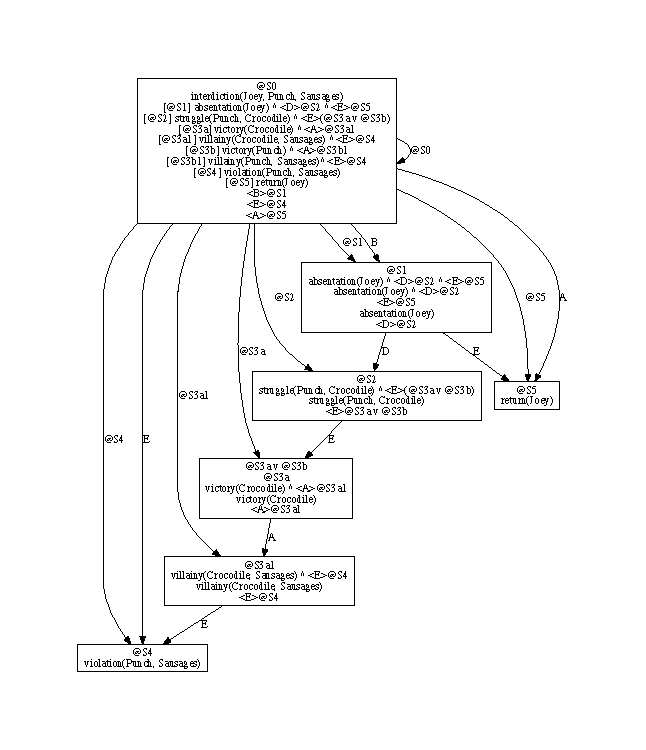
\includegraphics[width=0.9\textwidth]{crocmodel.pdf}}
  \caption{One model from the sausages scene in LoTREC}\label{fig:lotrec}
\end{figure}

We use Kripke structures \cite{kripke1963semantical} as a method of interpreting the combination of modal logic with Interval Temporal Logic. A Kripke structure is a graph, the nodes of which represent a possible world consisting of a set of assertions, and the edges of which are the accessibility relations between worlds.

\subsubsection{LoTREC}
% Read the book
In order to build and visualise the Kripke structures, we use LoTREC \cite{del2001lotrec}, a generic tableaux prover for modal and description logics. It allows the user to build up Kripke models using a domain specific language and display those models in the form of a graph diagram.
LoTREC uses the tableau method for model checking. This method checks whether or not its input is satisfiable by attempting to build a model for it. If the model construction fails, then the input is unsatisfiable.
Building models in LoTREC consists of defining \emph{connectors}, \emph{rules} and \emph{strategies}. Connectors are the logical operators used in formulas, rules are the instructions LoTREC needs to expand them into new nodes and edges and strategies are ways of combining rules in order to form models.
LoTREC takes an initial set of formulas as input and expands each formula into its components. These formulas are input using a simple prefix notation domain specific language consisting of operators and arguments, described in the LoTREC instruction book \emph{Kripke's Worlds} \cite{gasquet2013kripke}.
In the expansion, if a $[\,]$ (necessary) operator is encountered, then the formulas that serve as its argument are propagated across to all subsequent nodes. In the case of a $\langle \, \rangle$ (possibility) operator, a new node (possible world) is created containing its arguments. In both cases, binary operators can be used where one argument is located inside the square or angle brackets. In these cases, the argument inside the brackets is the accessibility relation, and is used to label the edges leading to the subsequent nodes.
In the case of a disjunction ($\lor$) operator, the current model is copied in its entirety and extended with one of the operator's arguments. The other argument is added onto the current model. This is an important way of creating alternative routes through the narrative, all of which can be checked for consistency.

\paragraph{The Sausages Scene in LoTREC}
The narrative is captured as a system of interval temporal logic assertions over story functions. The  assertions are interpreted using a tableaux reasoner by unpacking them to form a Kripke structure.
Using the initial formulas from figure \ref{fig:situations} as input, figure \ref{fig:lotrec} shows the model for the case where Punch wins the fight with the Crocodile. One other model exists in this scenario, in which the Crocodile is instead the victor.

The example in figure \ref{fig:lotrec} describes the fabula of a branching story, where either Punch or the Crocodile may win the fight for the sausages. This corresponds to the disjunction in figure \ref{fig:situations}, formula \ref{eq:struggle}. This leads to the creation of two models: the one in which the Crocodile wins and then goes on to eat the sausages (situation $@S_{3a}$), and the one in which Punch wins (situation $@S_{3b}$).
Using a breadth first strategy like LoTREC we would build all models simultaneously. This enables them to be checked for internal consistency, eliminating potentially impossible temporal arrangements. For example, no interval may come after or later than itself.

The first node contains the logical description of the story, which is then unpacked into subsequent nodes. It starts with the initial situation, $S_0$, which contains an interdiction: $\mathit{interdiction(Joey, Punch, Sausages)}$, where Joey tells Punch to look after the sausages. The other situations, $S_1$ to $S_5$ are listed using the necessity operator, with their accessibility relations being each situation's nominal operator (such as $@S_1$). This means that these situations are all created as new nodes, linked to the root node using their nominal accessibility relation, and so can be referred to later using the nominal operator. In this way, situations can refer to other situations.

For example, in Propp's formalism, an interdiction must begin with the absentation of a character and end with the interdiction's violation. For this reason, the initial situation is connected to $@S_1$, ($\mathit{absentation(Joey)}$), with the $\langle B \rangle$ (begins) accessibility relation and to $@S_4$, ($\mathit{violation(Punch, Sausages)}$), with the $\langle E \rangle$ (ends) accessibility relation. As other situations are unpacked into nodes, they are linked to other situations in the same way. An example of this is shown in $S_1$, the absentation, which must end with Joey's return, $S_5$, and during which a struggle must occur ($S_2$). As the formulas inside $S_1$ are unpacked, $S_1$ is linked to the other situations with the appropriate temporal accessibility relations. This is all made possible with the hybrid logic, which allows nodes to be referred to by name and linked to.

By describing situations that are linked together with temporal relations, we can build narratives and check them as we go. If a narrative is inconsistent in some way (by stating that a character is both dead and alive, for example), then the model will be unsatisfiable. This is useful for ensuring the construction of consistent narratives.

Additionally, every time a story has the possibility of branching off, the model for each new branch can be checked to see if it is viable in the narrative world. This means that rather than relying on an author to write out each branch of a story, they can be generated automatically from a story description and checked for inconsistencies.

As mentioned previously, the combination of Interval Temporal Logic and a narrative formalism such as Propp's allows us to create abstracted story components. For example, we have described the interdiction as being started by an absentation and ended with a violation. This pattern can be called the ``interdiction pattern'', and so can be easily reused in other narratives.

The use of LoTREC has shown the utility of being able to visualise a branching narrative in its entirety. This suggests that our method enables the visual authoring of interactive narratives by non-technical creators. Rather than having to type in computer code, or logical formulas, a visual tool could be developed to create logically consistent narrative worlds.

This approach for describing narrative has many potential real-world uses. One obvious use would be for computer game narratives, but it could also be used to describe a repeatable training scenario, and the possible choices available to a user at any point during the simulation.

\subsection{Deontic Logic and Norms}

\section{Norms and Institutions}
\label{sec:norms-and-institutions}

An institution describes a set of `social' norms describing the permitted and obliged behaviour of interacting agents. Noriega's `Fish Market' thesis~\cite{noriega1999agent} describe how an institutional model can be used to regiment the actions of agents in a fish market auction. Several~\cite{artikis2009specifying,fornara2007agent,cardoso2007institutional} extend this idea to build systems where institutions actively regulate the actions of agents, while still allowing them to decide what to do. We build on the work of Cliffe et al.~\cite{cliffe2007specifying} and Lee et al.~\cite{lee2013decoupling} to adapt it for the world of narrative, using an institutional model to describe the story world of Punch and Judy in terms of Propp's story moves and character roles, through which the actors acquire powers and permissions appropriate to the character and the story function in which they are participating.

Institutional models use concepts from deontic logic to provide obligations and permissions that act on interacting agents in an environment. By combining this approach with Propp's concepts of \emph{roles} and \emph{story moves}, we describe a Propp-style formalism of Punch and Judy in terms of what agents are \emph{obliged} and \emph{permitted} to do at certain points in the story.

For example, in one Punch and Judy scene, a policeman enters the stage and attempts to apprehend Punch. According to the rules of the Punch and Judy world, Punch has an obligation to kill the policeman by the end of the scene (as this is what the audience expects to happen, having seen other Punch and Judy shows). The policeman has an obligation to try his best to catch Punch. Both agents have permission to be on the stage during the scene. The policeman only has permission to chase Punch if he can see him (Punch is obliged to hide from him at the start of the scene).

The permissions an agent has, on the one hand, constrain the choices of actions available to them at any given moment. Obligations, on the other hand, affect the goals of an agent. Whether or not an agent actively tries to fulfil an obligation depends on their emotional state.

\subsection{Institution example}
To illustrate the application of institutional modelling, we here continue the `sausages and crocodile' scene example from section~\ref{sec:pjexample}, taking the Propp story functions and describing them in an institutional model.  We define our institution in terms of \emph{fluents}, \emph{events}, \emph{powers}, \emph{permissions} and \emph{obligations}, following~\cite{cliffe2007specifying}, to which the interested reader is referred for the full details of the formal model, including the generate ($\cal G$) and consequence ($\cal C$) relations, which are only described here in sufficient depth for the model being presented.

\subsubsection{Fluents}
These are properties that may or may not hold true at some instant in time, and that change over the course of time. \emph{Institutional events} are able to \emph{initiate} or \emph{terminate} fluents at points in time. A fluent could describe whether a character is currently on stage, the scene of the story that is currently being acted out, or whether or not the character is happy at that moment in time.
Domain fluents ($\mathcal{D}$) describe domain-specific properties that can hold at a certain point in time. In the Punch and Judy domain, these can be whether or not an agent is on stage, or their role in the narrative: % (equation~\ref{eq:domain}).
\begin{align*}
   \mathcal{D} &= \left\{\mathtt{onstage, hero, villain, victim, donor, item}\right\} %\label{eq:domain}
\end{align*}

Institutional fluents consist of (institutional) \emph{powers}, \emph{permissions} and \emph{obligations}.
% check your facts on this one
An \textbf{institutional power} ($\mathcal{W}$) describes whether or not an external event has the authority to generate a meaningful institutional event. Taking an example from Propp's formalism, an \emph{absentation\/} event can only be generated by an external event brought about by a \emph{donor\/} character (such as their leaving the stage). Therefore, any characters other than the donor character would not have the institutional power to generate an \emph{absentation\/} institutional event when they leave the stage.
The possible empowerments (institutional events) from Propp used in Punch and Judy are:
\begin{align*}
  \mathcal{W} =&\left\{\mathtt{pow(introduction), pow(interdiction), pow(give),}\right.\\ %\nonumber\\
               &\left. {} \mathtt{pow(absentation), pow(violation), pow(return)}\right\} %\label{eq:power}
\end{align*}

\subsubsection{Permissions} ($\mathcal{P}$) are associated with external actions that agents are permitted to do at a certain instant in time. These can be thought of as the set of \emph{socially permitted\/} actions available to an agent. While it is possible for an agent to perform other actions, societal norms usually discourage them from doing so.
% PJ examples
For example, it would not make sense in the world of Punch and Judy if Punch were to give the sausages to the Policeman. It is always Joey who gives the sausages to Punch. Also, it would be strange if Joey were to do this in the middle of a scene where Punch and Judy are arguing. We make sure agents' actions are governed so as to allow them only a certain subset of permitted actions at any one time. The set of permission fluents is:
\begin{align*}
\mathcal{P} =& \left\{\mathtt{perm(leavestage), perm(enterstage), perm(die), perm(kill),}\right.\nonumber\\
             &\left. {} \mathtt{perm(hit), perm(give), perm(fight)}\right\} %\label{eq:perm}
\end{align*}

\subsubsection{Obligations} ($\mathcal{O}$) are institutional facts that contain actions agents \emph{should} do before a certain deadline. If the action is not performed in time, a \emph{violation event} is triggered, which may result in a penalty being incurred. While an agent may be obliged to perform an action, it is entirely their choice whether or not they actually do so. They must weigh up whether or not pursuing other courses of action is worth accepting the penalty that an unfulfilled obligation brings.

% replace with sausages obligation
Anybody who has seen a Punch and Judy show knows that at some point Joey tells Punch to guard some sausages, before disappearing offstage. Joey's departure is modelled in the institution as the \emph{absentation\/} event. It could also be said that Joey has an obligation to leave the stage as part of the \emph{absentation} event, otherwise the story function is violated. This can be described in the institution as:
\begin{align*}
  \mathcal{O} =& \left\{\text{obl}(\mathtt{leavestage, absentation, viol(absentation)})\right\}%\label{eq:obl}
\end{align*}
The first argument is the external event that must be triggered according to the obligation, the second argument is the institutional deadline event, and the third argument is the violation event which is triggered if the obligation is not fulfilled before the deadline. 

\subsubsection{Events}
% actually 3 kinds, including violation events
Cliffe's model specifies three types of \textbf{event}: \emph{external events} (or `observed events', $\mathcal{E}_{obs}$), \emph{institutional events} ($\mathcal{E}_{instevent}$) and \emph{violation events} ($\mathcal{E}_{viol}$). Examples of each are given in Figure~\ref{fig:events}.
\emph{External events} are observed to happen in the agents' environment, which can \emph{generate} \emph{institutional events} which occur only within the institional model, leading to the \emph{initiation} or \emph{termination} of (domain) fluents, permissions, obligations or institutional powers.
An external event could be an agent leaving the stage, an agent hitting another, or an agent dying. Internal events include narrative events such as scene changes, or the triggering of Propp story functions such as \emph{absentation} or \emph{interdiction} (described in section~\ref{sec:propp}). \emph{Violation} is the name of a Propp story function, and is included as an internal event, although it has no relation to the violation events of an institution.
Violation events occur when an agent has failed to fulfil an obligation before the specified deadline. These can be implemented in the form of a penalty, by decreasing an agent's health, for example.

\begin{figure}[!t]
\begin{align}
  \mathcal{E}_{obs} =& \left\{\mathtt{startshow, leavestage, enterstage, die, give,}\right.\nonumber\\
  &\left. {} \mathtt{harmed, hit, fight, kill, escape}\right\}\label{eq:eobs}\\
  \mathcal{E}_{instevent} =& \left\{\mathtt{introduction, interdiction, receipt, absentation,}\right.\nonumber\\
                         &\left. {} \mathtt{violation, return, struggle, defeat, complicity,}\right.\nonumber\\
                         &\left. {} \mathtt{victory, escape}\right\}\label{eq:einst}\\
  \mathcal{E}_{viol} =& \left\{\mathtt{viol(introduction), viol(interdiction), viol(receipt),}\right.\nonumber\\
 &\left. {} \mathtt{viol(absentation), viol(violation), viol(return),}\right.\nonumber\\
 &\left. {} \mathtt{viol(struggle), viol(defeat), viol(complicity)}\right.\nonumber\\
 &\left. {} \mathtt{viol(victory), viol(escape)}\right\}\label{eq:viol}
\end{align}
\caption{External, institutional and violation events for Punch and Judy} \label{fig:events}
\end{figure}

% internal and external

\subsubsection{Event Generation and Consequences}
An \textbf{event generation} function, $\mathcal{G}$, describes how events
($\mathcal{E}$, usually external, but can also be internal) %\mnote{Added $\mathcal{E}$ explanation here}
can generate other (usually institutional) events, conditional upon the current institutional state ($\cal X$). This is the counts-as relation.  For example, if an agent leaves the stage while the \emph{interdiction} event holds, they trigger the \emph{leavestage} event. This combination generates the \emph{absentation} institutional event (rule~\ref{eq:absentation}). Further examples appear in figure~\ref{fig:gen}.

Event generation functions follow a $\langle \mathtt{preconditions} \rangle \rightarrow \{\mathtt{postconditions}\}$ format. The preconditions consist of a set of fluents that hold at that time, along with an event to have occurred. The postconditions are the events that are generated. The generation functions are used to generate internal, institutional events from external events.

Consider the Punch and Judy scenario described in section~\ref{sec:pjexample}. There are seven institutional events (story functions) that occur during this scene: \emph{interdiction}, \emph{complicity}, \emph{receipt} (from Propp's \emph{receipt of a magical agent}) \emph{absentation}, \emph{violation}, \emph{struggle}, \emph{return}.
These institutional events are all generated by external events. The \emph{interdiction} is generated when Joey tells Punch to protect the sausages. Punch agreeing amounts to \emph{complicity}. Joey \emph{gives} punch the sausages (\emph{receipt}), then leaves the stage (\emph{absentation}). The crocodile eating the sausages is a \emph{violation} of Punch's oath, the agents fight (\emph{struggle}), then Joey enters the stage again (\emph{return}).

It is desirable that these story functions occur in this sequence in order for a satisfying narrative to emerge. Agents may decide to perform actions that diverge from this set of events, but the institution is guiding them towards the most fitting outcome for a \emph{Punch and Judy} world. For this reason, a currently active story function can be the precondition for event generation. For example, the \emph{receipt} event may only be triggered if an agent externally performs a \emph{give} action \textbf{and} if the \emph{complicity} event currently holds (rule~\ref{eq:receipt}).
Examples of event generation function for this scenario, complete with preconditions, are listed in rules~\ref{eq:gfirst}--\ref{eq:glast} (Figure~\ref{fig:gen}).

\begin{figure}[!t]
\abovedisplayskip=0pt
\abovedisplayshortskip=0pt
$\mathcal{G(X, E)}:\left\{\mbox{%
{\begin{minipage}[c]{0.85\textwidth}
% \vspace{-2.1em}\begin{align}
\begin{align}
\langle \emptyset,\mathit{tellprotect}\mathtt{(donor, villain, item)} \rangle%\nonumber\\
             %         &\qquad\qquad\qquad
& \rightarrow \left\{\mathit{interdiction}\right\}\label{eq:gfirst}\\
                      \langle \{\mathit{interdiction}\}, \mathit{agree}\mathtt{(villain)}) \rangle %\nonumber\\
            %          &\qquad\qquad\qquad
& \rightarrow \left\{\mathit{complicity}\right\}\\
                      \langle \emptyset, \mathit{give}\mathtt{(donor, villain, item)}) \rangle %\nonumber\\
        %              &\qquad\qquad\qquad
& \rightarrow \left\{\mathit{receipt}\right\}\label{eq:receipt}\\
                      \langle \{\mathit{interdiction}\}, \mathit{leavestage}(\mathtt{donor}) \rangle %\nonumber\\
              %        &\qquad\qquad\qquad
& \rightarrow \left\{\mathit{absentation}\right\}\label{eq:absentation}\\
                      \langle \{\mathit{interdiction}\}, \mathit{harmed}(\mathtt{item}) \rangle %\nonumber\\
         %             &\qquad\qquad\qquad
& \rightarrow \left\{\mathit{violation}\right\}\\
                      \langle \{\mathit{interdiction, absentation}\},
                      \mathit{enterstage}(\mathtt{donor}) \rangle %\nonumber\\
              %        &\qquad\qquad\qquad
& \rightarrow \left\{\mathit{return}\right\}\\
                      \langle \emptyset, \mathit{hit}(\mathtt{donor, villain}) \rangle %\nonumber\\
%                      &\qquad\qquad\qquad
& \rightarrow \left\{\mathit{struggle}\right\}\label{eq:glast}
\end{align}
\end{minipage}}}\right.$
\caption{Event generation in the sausage scene} \label{fig:gen}
\end{figure}

\textbf{Consequences} consist of fluents, permissions and obligations that are \emph{initiated} ($\mathcal{C}^{\uparrow}$) or \emph{terminated} ($\mathcal{C}^{\downarrow}$) by institutional events. For example, the institutional event \emph{receipt} initiates the donor agent's permission to leave the stage, triggering the \emph{absentation} event (rule~\ref{eq:initgive}). When the \emph{interdiction} event is currently active and a \emph{violation} event occurs, the interdiction event is terminated (\ref{eq:interm}). Rules~\ref{eq:cfirst}--\ref{eq:clast} in Figures~\ref{fig:init} and~\ref{fig:term} describe the initiation and termination of fluents in the Punch and Judy sausages scene detailed in section~\ref{sec:pjexample}.

\begin{figure}[!t]
\abovedisplayskip=0pt
\abovedisplayshortskip=0pt
$\mathcal{C^{\uparrow}(X, E)}:\left\{\mbox{%
\begin{minipage}[c]{0.85\textwidth}
\begin{align}
    \langle \emptyset, \mathtt{interdiction} \rangle %\nonumber\\
                                 % &\qquad\qquad
&\rightarrow \{\text{active}(\mathtt{interdiction}), \nonumber\\&\qquad\text{perm}(\mathtt{give(donor, villain, item)})\}\label{eq:cfirst}\\
                                 \langle \emptyset, \mathtt{receipt} \rangle % \nonumber\\
                                 % &\qquad\qquad
&\rightarrow \{\text{perm}(\mathtt{leavestage(donor)})\}\label{eq:initgive}\\
                                 \langle\{\mathit{active(absentation)}\}, \nonumber\\\mathtt{enterstage(villain)} \rangle %\nonumber\\
                                 %&\qquad\qquad
&\rightarrow \{\text{obl}(\mathtt{eat(villain, sausages),} \nonumber\\&\qquad\qquad\mathtt{return, viol(violation)})\}\label{eq:obl1}\\
                                 \langle\{\mathit{active(interdiction)}\}, \nonumber\\\mathtt{leavestage(donor)} \rangle % \nonumber\\
                                 % &\qquad\qquad
&\rightarrow \{\text{obl}(\mathtt{enterstage(donor),}\nonumber\\&\qquad\qquad\mathtt{eat(villain, sausages),}\nonumber\\&\qquad\qquad\mathtt{viol(return)})\}\label{eq:obl2}\\
                                 \{\mathit{active(interdiction)}\},\nonumber\\ \mathtt{violation} \rangle %\nonumber\\
                                 % &\qquad\qquad
&\rightarrow \{\text{perm}(\mathtt{enterstage(dispatcher)})\}\\
                                 \langle\{\mathit{active(absentation),}\nonumber\\\mathit{active(violation)}\},\nonumber\\ \mathtt{return} \rangle %\nonumber\\
                                 %&\qquad\qquad
&\rightarrow \{\text{perm}(\mathtt{hit(donor, villain)})\}
\end{align}
\end{minipage}}\right.$
\caption{Fluent initiation in the sausage scene} \label{fig:init}
\medskip
\abovedisplayskip=0pt
\abovedisplayshortskip=0pt
$\mathcal{C^{\downarrow} (X, E)}:\left\{\mbox{%
\begin{minipage}[c]{0.85\textwidth}
\begin{align}
\langle \emptyset, \mathtt{interdiction} \rangle %\nonumber\\
                                   %&\qquad\qquad
&\rightarrow \{\text{perm}(\mathtt{give(donor, villain, item)})\}\\
                                   \langle \{\mathit{active(interdiction)}\},\nonumber\\ \mathtt{absentation} \rangle %\nonumber\\
                                   %&\qquad\qquad
&\rightarrow \{\text{perm}(\mathtt{leavestage(donor)})\}\\
                                   \langle \{\mathit{active(interdiction)}\},\nonumber\\ \mathtt{violation} \rangle %\nonumber\\
                                   %&\qquad\qquad
&\rightarrow \{\mathit{active(interdiction)}\}\label{eq:interm}\\
                                   \langle \{\mathit{active(absentation),}\nonumber\\\mathit{ active(violation)}\},\nonumber\\ \mathtt{return} \rangle %\nonumber\\
                                   %&\qquad\qquad
&\rightarrow \{\mathit{active(absentation)}\}\label{eq:clast}
\end{align}
\end{minipage}}\right.$
\caption{Fluent termination in the sausage scene} \label{fig:term}
\end{figure}%\mnote{Added \emph{active(interdiction)} to top of fig. \ref{fig:init}}

\section{Why Use Institutions for Interactive Narrative?}
\label{sec:why-use-institutions}
% Write about character freedom, regimentation vs regulation. Give story
% examples vs using a planner

\section{Modelling of Coordinated Instutions}
% Put bridge institution stuff here
